\chapter{数据}
\label{cha:data}
在本章中,我们将介绍本文中使用的数据集,包括一些公开数据集如Restaurant,Laptop,Twitter以及我们所构建的新闻驱动的股票预测数据集senti-stock。
\section{SemEval 2014 Task 4}
SemEval 2014 Task 4是一个基于方面的情感分析数据集,是在基于方面的情感分析领域应用最为广泛的数据集。基于方面的情感分析旨在提取句子中对某一方面或目标的情感极性。这一数据集由人工标注的餐厅Restaurant和笔记本电脑Laptop的评论组成。数据集分为训练集和测试集两部分。从表中的数据可以看出,在训练集和测试集中,积极、消极、中性的标签分布并不均衡,尤其是笔记本电脑Laptop评论数据集。同时,训练数据的量并不是很大。这些特点给这一数据集增加了难度。Restaurant和Laptop数据集都是一个比较正式的数据,句子都比较完整,语法较规范。

\begin{table}[ht]
	\centering
	\caption{SemEval 2014 Task 4数据集统计信息}
	\label{tab:stat}
	\begin{tabular}{|l|l|l|l|}
	\hline
	Dataset & Positive & Negative & Neutral\\
	\hline
	Laptop-Train &  994 & 870 & 464\\
	Laptop-Test & 341 & 128 & 169\\
	Restaurant-Train & 2164 & 807 & 637\\
	Restaurant-Test & 728 & 196 & 196\\
	% Twitter-Train & 1567 & 1563 & 3127 \\
	% Twitter-Test & 174 & 174 & 346 \\
	\hline
	\end{tabular}
\end{table}
表~\ref{tab:stat}显示了Restaurant和Laptop数据集的统计信息。
\section{Twitter}
Twitter~\cite{dong2014adaptive}是一个由推特内容构成的数据集。这个数据集针对于对某一目标的情感分析问题,是由人工标注的。表~\ref{tab:twitterdataset}显示了该数据集的统计信息。推特Twitter数据集分为训练集和测试集两部分,从表\ref{tab:twitterdataset}中可以看出,推特Twitter数据集中训练集和测试集的标签分布相对来说还是比较均匀的。但推特数据集中的句子多比较口语化,涉及很多口语化的表达,句式不规范,甚至包含emoji表情等内容,这些都给这一数据集增加了难度。
\begin{table}[ht]
	\centering 
	\caption{Twitter数据集统计信息}
	\label{tab:twitterdataset}
	\begin{tabular}{|l|l|l|l|}
	\hline
	Dataset & Positive & Negative & Neutral\\
	\hline 
	% Laptop-Train &  994 & 870 & 464\\
	% Laptop-Test & 341 & 128 & 169\\
	% Restaurant-Train & 2164 & 807 & 637\\
	% Restaurant-Test & 728 & 196 & 196\\
	Twitter-Train & 1567 & 1563 & 3127 \\
	Twitter-Test & 174 & 174 & 346 \\
	\hline
	\end{tabular}
\end{table}
\section{senti-stock}

在之前的研究中用到的股票预测的数据集大都是不公开的。为此,我们构建了新闻驱动的股票预测数据集senti-stock并将其公开。本章将详细介绍我们如何收集数据、处理数据以及数据如何获取。图~\ref{fig:liuchengtu}显示了数据收集和处理的流程。

\begin{figure}[ht]
	\centering 
	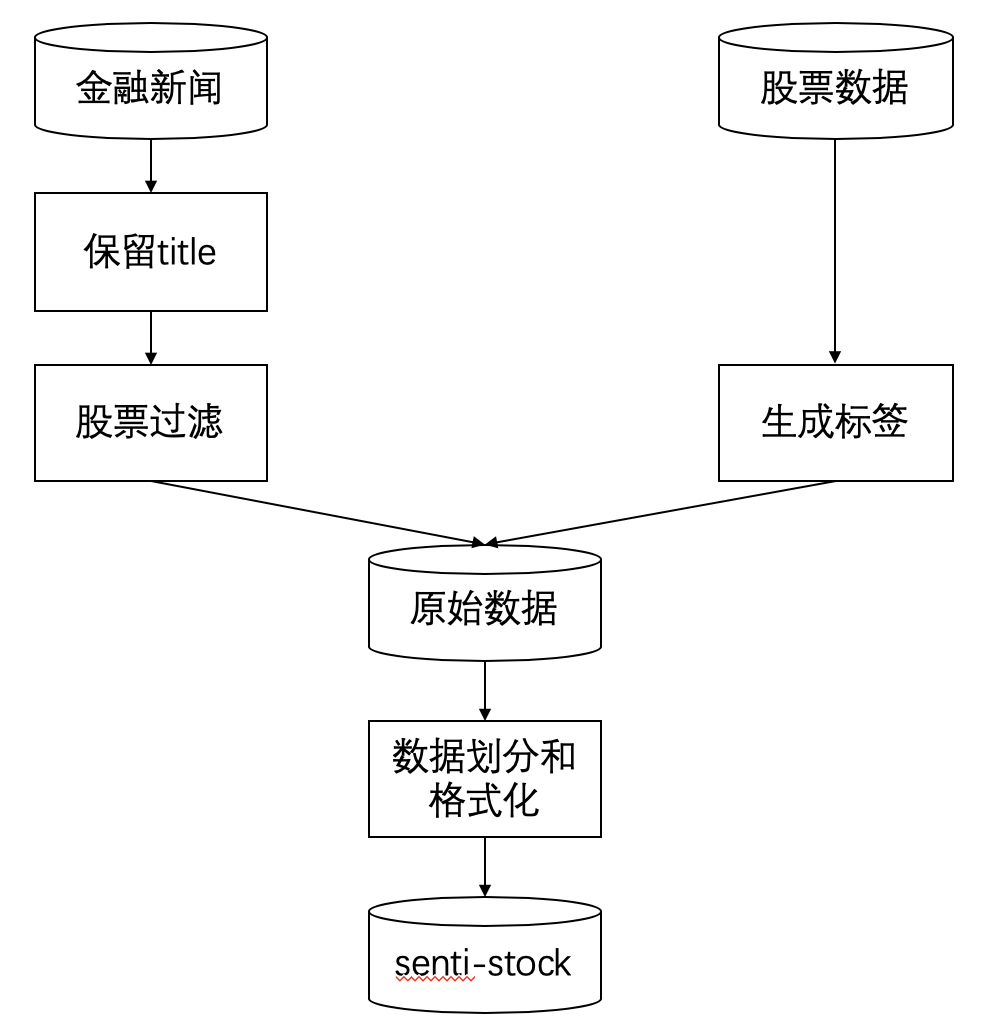
\includegraphics[width=0.5\linewidth]{LIUCHENGTU.png}
	\caption{senti-stock数据收集和处理流程图}
	\label{fig:liuchengtu}
\end{figure}

\subsection{收集数据}
我们选择美国股票市场作为研究对象。美国股市是指包含纽约证券交易所(New York Stock Exchange) 及纳斯达克证券市场 (Nasdaq Stock Market) 上市的股票 。道琼斯工业股票指数、纳斯达克指数和标准普尔500指数三大股指代表着美国股市的兴衰。美国股票市场于1811年建立,至今已经有两百年的历史。十八世纪,美国股票市场得到了初步发展;十八世纪末到十九世纪初,美国股市进一步发展,但市场操纵和内幕交易情况严重;十九世纪中期以前,美国股票市场进入规范化的发展时期;十九世纪中期至今,机构投资发展迅速,美国股票市场进入现代投资时代。因为其历史悠久,美国股票市场目前已经处于一个比较规范化的发展阶段。纽约证券交易所有超过三千支股票,包括一些历史悠久的大型企业,股份总值达到七兆亿美元;纳斯达克证券交易所是一个虚拟交易所,虽然历史较短,但有超过五千支股票,股票公司多为小型新公司。美国市场具有以下特点:
\begin{itemize}
	\item 规模大、市场成熟、运作规范、股价稳定;
	\item 证券市场管理严格、规范;
	\item 美国允许外国股份公司在美国证券市场发行股票并进行交易。
\end{itemize}

美国股票市场交易时间是周一到周五,美股没有单日股票涨跌幅限制,实行T+0交易制度,当天买入的股票可以当天卖出。
正因为美国股票市场具有上述特点,美国股票市场比中国股票市场更适合用来作为研究对象。

\begin{figure}[H]
	\centering 
	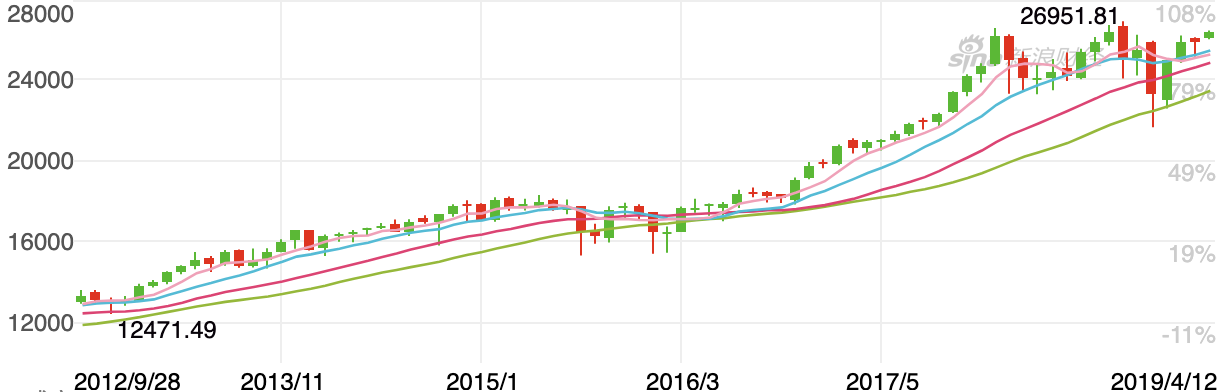
\includegraphics[width=0.8\linewidth]{djia.png}
	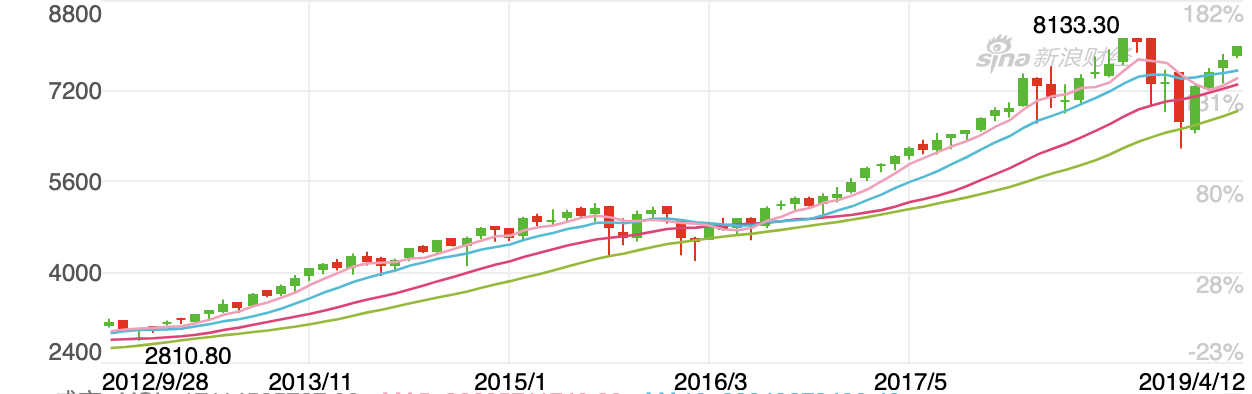
\includegraphics[width=0.8\linewidth]{nasdaq.png}
	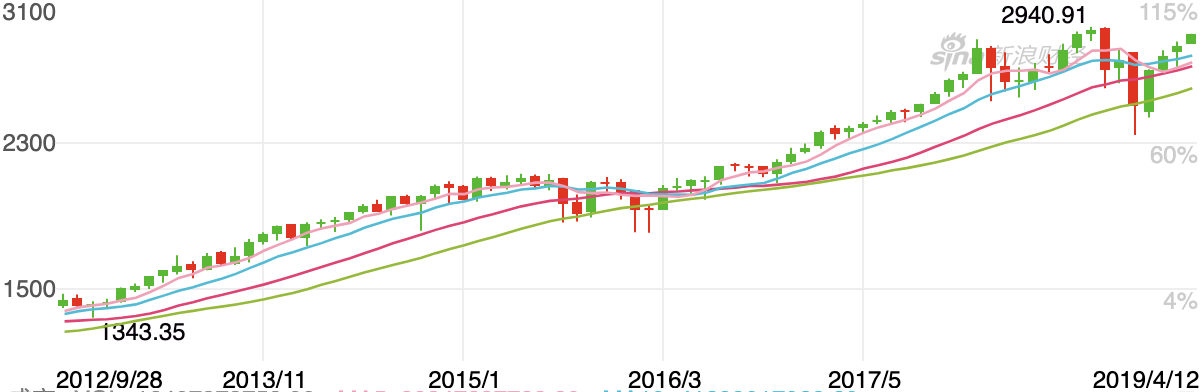
\includegraphics[width=0.8\linewidth]{sp500.png}
	\caption{美国市场三大指数:道琼指数、纳斯达克指数、标普500的月均线,图片来自新浪财经}
	\label{fig:index}
\end{figure}

\begin{table}[ht]
    \centering
    \begin{minipage}[t]{0.8\linewidth}
    	\caption[]{新闻样例}
    	\label{tab:newsexample}
    	\begin{tabularx}{1\linewidth}{lX}
    		\toprule[1.5pt]
    		键 & 值 \\ \midrule[1pt]
    		news\_type & topStory \\ 
    		symbol & AMD \\ 
    		name & Advanced Micro Devices Inc \\ 
    		date & 20161020 \\ 
    		title & AMD revenue beats on demand for chips used in gaming consoles \\ 
    		content & Chipmaker Advanced Micro Devices Inc reported a better-than-expected 23.2 percent increase in quarterly revenue helped by higher demand for graphics chips used in gaming consoles. \\ 
    		\bottomrule[1.5pt]
    	\end{tabularx}
    \end{minipage}
\end{table}

我们主要从路透社收集新闻数据,从雅虎财经收集股票历史价格数据。

路透社(Reuters)是世界上最早创办的通讯社之一,也是目前英国最大的通讯社和西方四大通讯社之一。路透社是世界前三大的多媒体新闻通讯社,提供各类新闻和金融数据,在128个国家运行。路透提供新闻报导给报刊、电视台等各式媒体,并向来以迅速、准确享誉国际。雅虎财经提供金融新闻、数据、评论等内容,包括股票历史数据、金融新闻报道和原创内容。雅虎财经提供的股票历史数据以准确及时而著称,并且雅虎财经提供了方便使用的数据接口。

为了从路透社网站和雅虎财经网站上抓取数据,我们使用了Scrapy框架。Scrapy\footnote{https://pypi.org/project/Scrapy/}是一个为了爬取网站数据,提取结构性数据而编写的应用框架。它可以应用在包括数据挖掘,信息处理或存储历史数据等一系列的程序中。其最初是为了 页面抓取 (更确切来说, 网络抓取)所设计的, 也可以应用在获取API所返回的数据(例如 Amazon Associates Web Services) 或者通用的网络爬虫。我们所使用的爬取数据的源码可以在github上获得\footnote{https://www.github.com/Cppowboy/stock\_data\_crawler}。

我们从路透社的网站上抓取了从2015年1月1日到2018年1月1日的美国市场的股票新闻数据。图~\ref{fig:index}显示了美国市场三大指数(道琼指数、纳斯达克指数、标普500指数)在近几年的变化波动趋势。可以看到,在2015年到2018年期间,美国股市整体上呈现稳定增长的趋势。我们得到了关于1297支股票的共计121096条新闻数据。这些新闻全部以JSON的格式保存。表~\ref{tab:newsexample}显示了我们一个新闻的样例。其中,news\_type指的是新闻的类型,包括"topStory"和"normal"两种。"symbol"是股票的代码。"name"是股票的全称。"date"是新闻的日期,格式为"\%Y\%m\%d"。"title"和"content"分别表示新闻的标题和内容。我们使用一个python包fix-yahoo-finance〜\footnote{https://pypi.org/project/fix-yahoo-finance/}来获取每支股票的历史价格数据。

\begin{lstlisting}[language={Python}]
	from pandas_datareader import data as pdr
	import fix_yahoo_finance as yf
	yf.pdr_override() 
	
	data = pdr.get_data_yahoo("SPY", start="2017-01-01", end="2017-04-30")
	data = pdr.get_data_yahoo(["SPY", "IWM"], start="2017-01-01", end="2017-04-30")
	\end{lstlisting}

上面给出的fix-yahoo-finance的示例代码,我们利用这一工具得到了历史数据。在这里,我们假设某支股票的涨跌公与前一天、周、月的相关新闻有关,不受其他因素的影响。然后从短期(天)、中期(周)、长期(月)三个时间间隔去生成输出的标签~\cite{ding2014using}。三种不同的时间间隔的标签构成了Short、Middle、Long三个不同的数据集。如果股票价格在下一天、周、月的涨幅超过1\%,则将标签设为$+1$;如果股票价格在下一天、周、月的跌幅超过1\%,则将标签设为$-1$;其他股票的标签设为$0$。

\subsection{处理数据}

之前的研究表明,新闻的标题更有助于预测新闻事件的影响,而新闻的内容往往包含太多不相关的信息。因此,我们只使用新闻的标题\cite{ding2014using}。
\begin{figure}[ht]
	\centering
	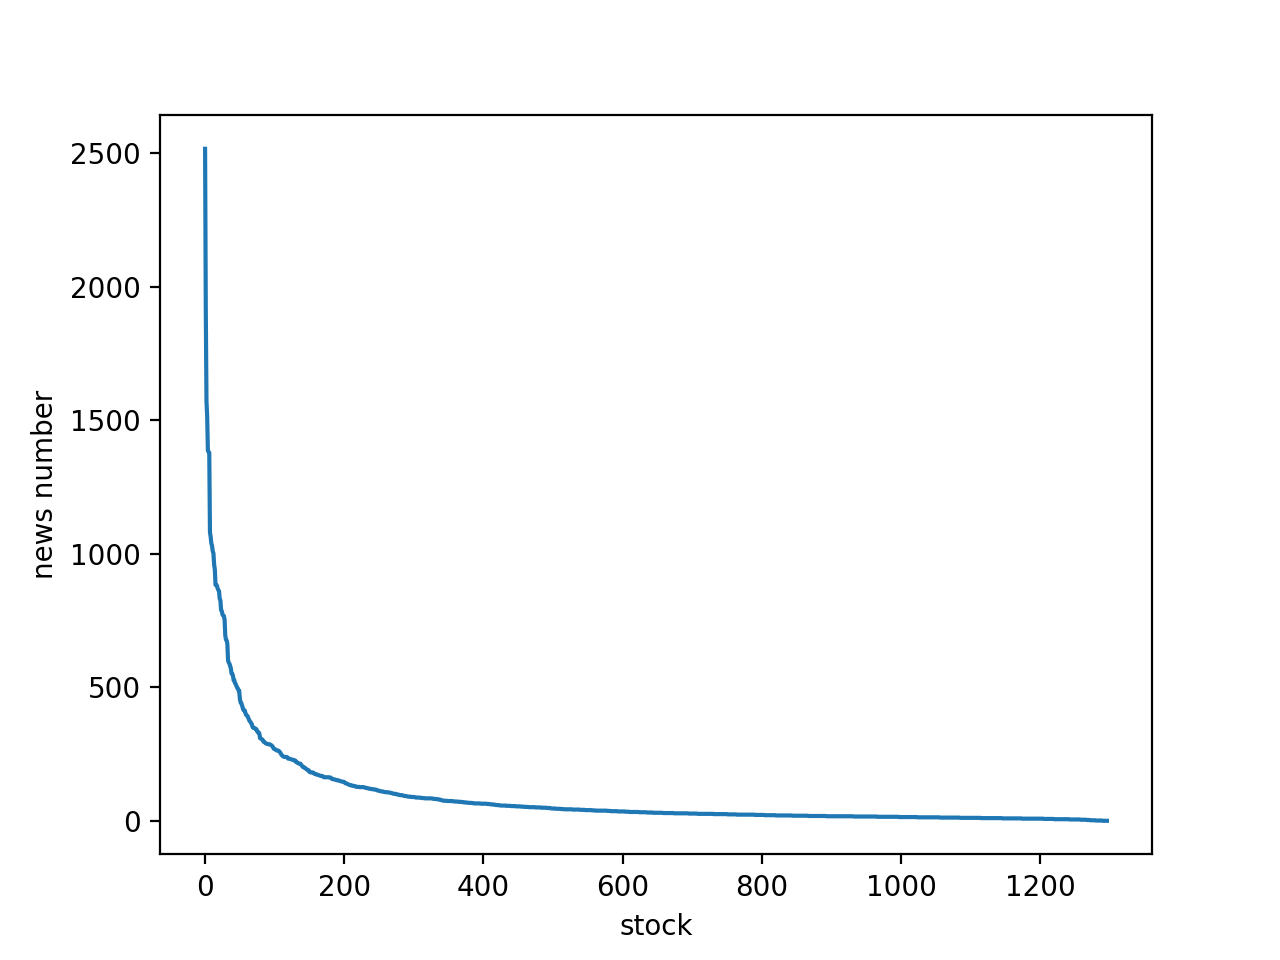
\includegraphics[width=0.8\linewidth]{all_stock_distribution.png}
	\caption{1297支股票的新闻数量分布}
	\label{fig:all-stock-distribution}
\end{figure}
图\ref{fig:all-stock-distribution}显示了全部股票的新闻数量分布。可以看到,大部分股票的相关新闻数量非常少,但有些比较知名的股票公司,其相关的新闻非常多。近期的研究\cite{ding2014using}显示,知名股票的预测准确率要高于不那么知名的股票,因为与知名股票相关的新闻事件数量更高。不知名股票的日常新闻非常少,以致于难以提取足够的信息来预测股票的变动。因此,我们对所有的股票进行简单的过滤,只保留新闻数量超过五百的股票,得到46支股票。这46支股票的新闻数量分布如图\ref{fig:good_stock_distribution}所示,这46支股票均是在美国市场中比较有知名度的股票。

\begin{figure}[ht]
	\centering 
	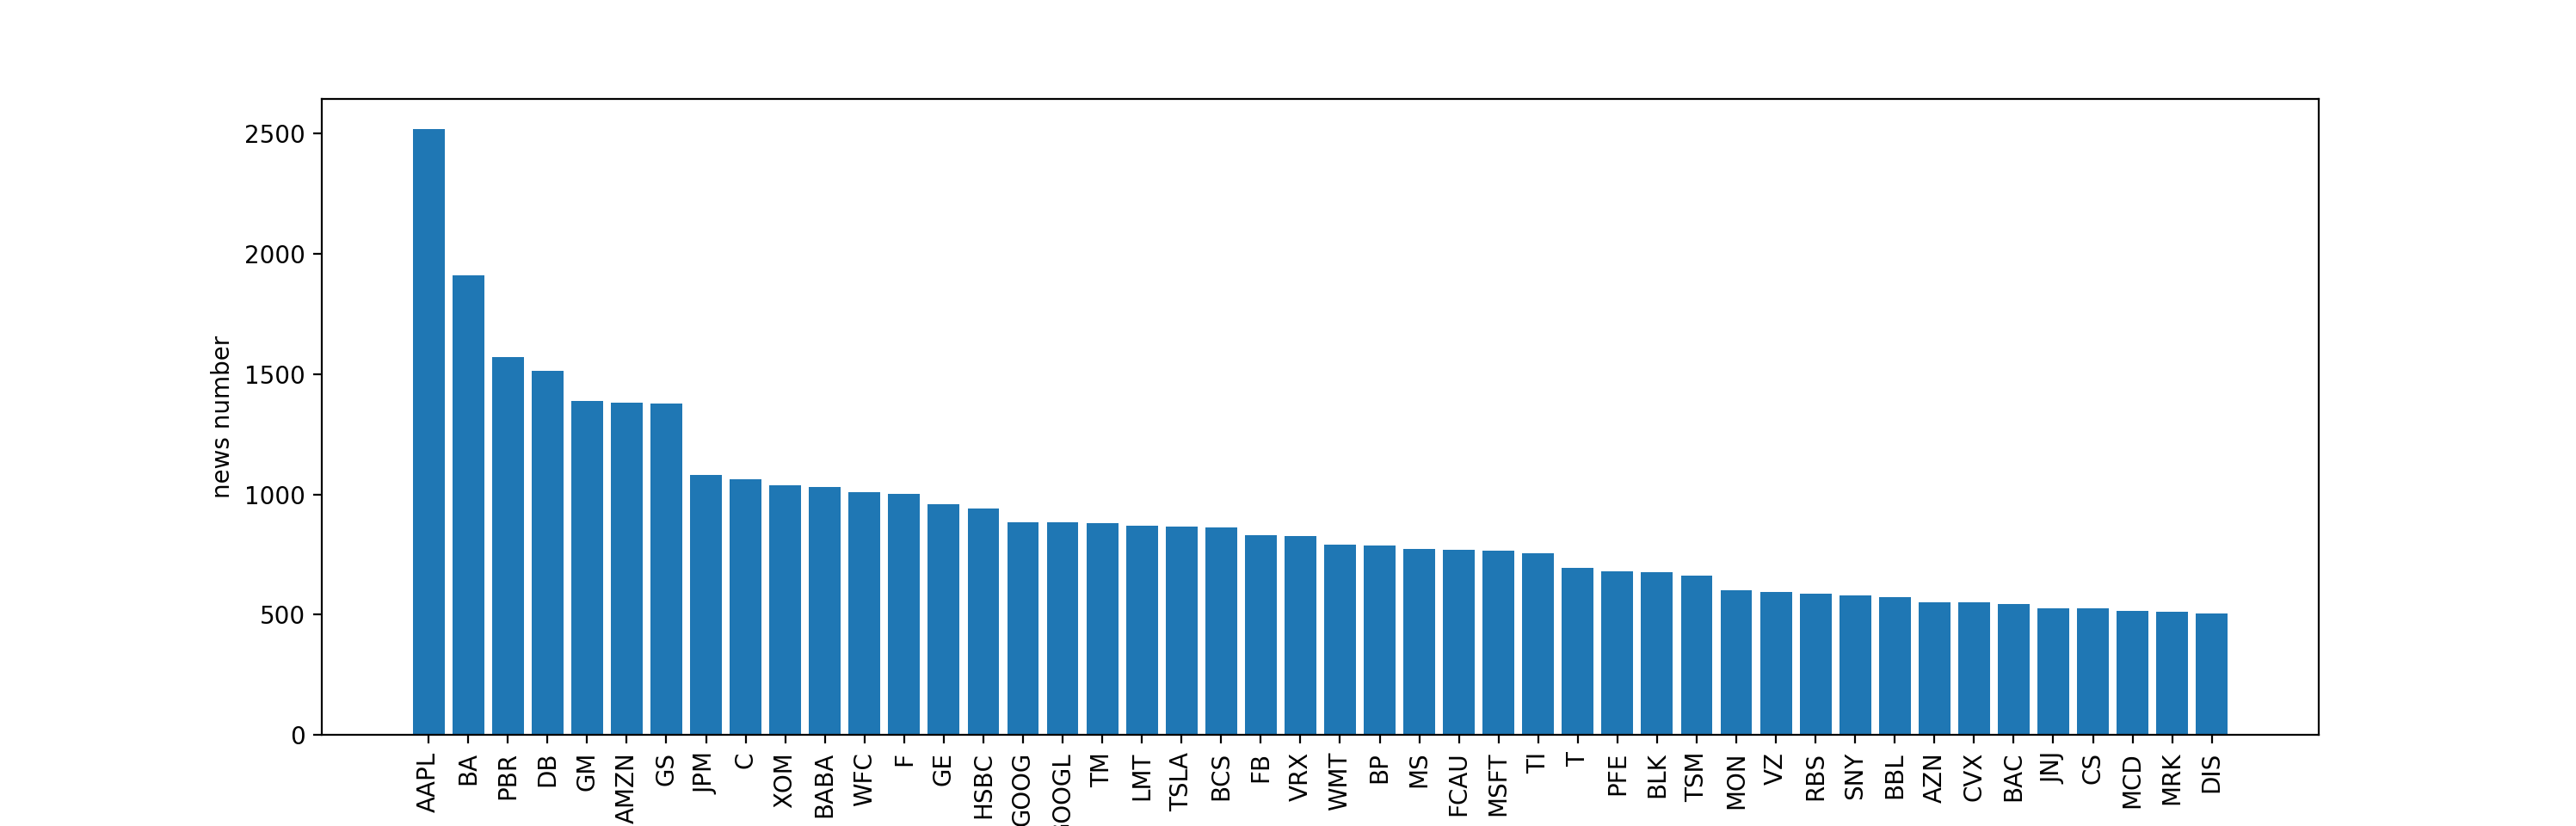
\includegraphics[width=\linewidth]{good_stock_distribution.png}
	\caption{新闻数超过五百的股票新闻数分布}
	\label{fig:good_stock_distribution}
\end{figure}

\begin{table}[ht]
	\centering 
	\begin{minipage}[t]{0.8\linewidth}
		\caption[]{数据集的统计信息}
		\label{tab:datasetstatistics}
		\begin{tabularx}{1\linewidth}{lXXX}
			\toprule[1.5pt]
			数据集 & 全部数据 & 多标签数据 & 困难数据\\ \midrule[1pt]
			Short-Train & 25496 & 3623 & 33 \\ 
            Short-Test & 6374 & 287 & 8 \\ 
            Middle-Train & 30637 & 4368 & 176 \\ 
            Middle-Test & 7660 & 353 & 17 \\ 
            Long-Train & 18324 & 2510 & 157 \\
			Long-Test & 4581 & 218 & 12 \\ 
			\bottomrule[1.5pt]
		\end{tabularx}
	\end{minipage}
\end{table}

在完成上述处理后,我们将数据按照4:1的比例划分为训练集和测试集。表\ref{tab:datasetstatistics}显示了数据集的一些统计信息。其中,多标签数据指的是同一条新闻有多支相关的股票;困难数据指的是同一条新闻有多支相关股票且这些股票的涨跌情况不同,即同一条新闻对不同的股票有着不同的影响。困难数据是多标签数据的一个子集。

\begin{table}[ht]
	\centering
	\begin{minipage}[t]{0.8\linewidth}
		\caption{数据集中标签的分布}
		\label{tab:labeldistribution}
		\begin{tabularx}{\linewidth}{lXXX}
			\toprule 
			& $+1$ & $0$ & $-1$ \\ \midrule  
			Short-Train & 5483 & 141915 & 5098 \\ 
			Short-Test & 1388 & 3640 &1346 \\
			Middle-Train & 11716 & 8743 & 10178 \\
			Middle-Test & 2936 & 2207 & 2517 \\ 
			Long-Train & 9109 & 2470 & 6745 \\ 
			Long-Test & 2194 & 653 & 1734\\ 
			\bottomrule
		\end{tabularx}
	\end{minipage}
\end{table}

表\ref{tab:labeldistribution}显示了数据集中各类标签的分布情况。在短期标签的数据集中,大部分标签的类别都是$0$。这是因为在很短的时间(一天)内,股票的价格往往不会出现较大的变动。中期标签的数据集比另外两个数据集要更加均衡。长期数据集中,大部分标签的类别都是$+1$,这是因为在2015年到2018年之间,股市整体上呈现稳定上升的趋势。在这三种标签的数据集中,短期数据集和和长期数据集各类标签分布相对比较不均匀,因此相对容易,而中期数据集相对困难一些。

\subsection{公开数据}

我们的数据集senti-stock将会以xml的形式存储,其存储格式与SemEval 2014数据集格式一致\cite{pontiki2014semeval-2014},数据集可以从github上下载\footnote{https://www.github.com/Cppowboy/senti-stock}。
